%!TEX encoding = UTF-8 Unicode
%!TEX root = ../compendium.tex

\chapter{Integrerad utvecklingsmiljö}\label{appendix:ide}

\section{Vad är en integrerad utvecklingsmiljö?}

En integrerad utvecklingsmiljö \Eng{integrated development environment, IDE} samlar ett flertal verktyg, inklusive en avancerad \textbf{editor} (se appendix \ref{appendix:edit}), för att skapa, köra och testa program. Det finns flera utvecklingsmiljöer att välja mellan, som kan användas för både Scala och Java.

En IDE ger stöd för auto-komplettering \Eng{auto completion} där tillgängliga metoder visas i en lista och resten av ett namn kan fyllas efter att du skrivit de första bokstäverna i namnet. En IDE kan hjälpa dig med formattering och även skapa skelettkod utifrån \textbf{kodmallar} \Eng{code templates}. Med \textbf{felindikering} \Eng{error highlighting} får du understrykning av vissa fel direkt i koden och ibland kan du även få hjälp med förslag på åtgärder för att rätta till enkla fel. Funktioner för \textbf{avlusning} \Eng{debugging} hjälper dig att felsöka medan du kör din kod. Med funktioner för \textbf{omstrukturering} \Eng{refactoring} av kod får du hjälp av editorn i samarbete med kompilatorn att göra omfattande strukturförändringar i många kodfiler samtidigt, t.ex. namnbyten med hänsyn taget till språkets synlighetsregler.  

Alla dessa avancerade funktioner kan öka produktiviteten avsevärt, men samtidigt tar de tid att lära sig och en IDE kan kräva mycket datorkraft och viss väntetid jämfört med en vanlig, fristående editor. I början kan all funktionalitet upplevas som överväldigande och det kan vara svårt att hitta i alla menyer och inställningar. Ska man bara skriva ett litet, enkelt program, eller göra några mindre ändringar, är det många som föredrar en fristående, snabbstartad kodeditor före en fullfjädrad, tungrodd IDE. Å andra sidan kan en IDE hjälpa till att upptäcka vad som finns i ett api och autokompletteringsfunktionen hjälpa stort när man upptäcker och experimenterar med en okänd kodmassa.




\section{Kojo}\label{appendix:kojo}

Kojo är en integrerad utvecklingsmiljö för Scala som är speciellt anpassad för nybörjare i programmering. Kojo används i LTH:s Science Center Vattenhallen för utbildning av grundskolelärare i programmering och vid skolbesök och annan besöksverksamhet, i vilken lärare och studenter vid LTH arbetar som handledare. 

Kursens första laboration genomförs med hjälp av Kojo, men Kojo kan med fördel användas som komplement till Scala REPL och annan IDE under hela kursens gång. Medan Scala REPL lämpar sig för korta kodsnuttar, och en fullfjädrad, professionell IDE har funktioner för att hantera riktigt stora programmeringsprojekt, passar Kojo bra för mellanstora program. I Kojo finns även lätttillgängliga bibliotek som gör tröskeln lägre att programmera rörlig grafik och enkla spel.    

\subsection{Installera Kojo}

Kojo är förinstallerat på LTH:s datorer och körs igång med kommandot \texttt{kojo}. För instruktioner om hur du installerar Kojo på din egen dator se här:\\
\href{http://www.lth.se/programmera/installera/}{lth.se/programmera/installera}

Kojo kräver att \texttt{java} finns på din dator. Eftersom du behöver tillgång till JDK i kursen, är lika bra att installera hela JDK direkt (och inte bara JRE), se vidare hur man gör detta i avsnitt \ref{appendix:compile:install-jdk}. 
%\href{http://www.kogics.net/kojo-download}{www.kogics.net/kojo-download}


\subsection{Använda Kojo}

När du startar Kojo första gången, välj ''Svenska'' i språkmenyn och starta om Kojo. Därefter fungerar grafikfunktionerna på svenska enligt tabell \ref{table:kojo:functions}.

Det finns även ett antal användbara kortkommando som du hittar i menyerna i Kojo. Undersök speciellt Ctrl+Alt+Mellanslag som ger autokomplettering baserat på det du börjat skriva.


{\small\renewcommand{\arraystretch}{1.45}
\begin{longtable}{@{}p{0.42\textwidth} p{0.55\textwidth}}

\caption{Några av sköldpaddans funktioner. Se även \href{http://lth.se/programmera}{lth.se/programmera}}\label{table:kojo:functions}\\

\emph{Svenska/Engelska} & \emph{Vad händer?}  \\ \hline
\code|sudda| \newline \code|clear| & Ritfönstret suddas \\
\code|fram| \newline \code|forward(25)| & Paddan går framåt 25 steg. \\
\code|fram(100)| \newline \code|forward(100)| & Paddan går framåt 100 steg. \\
\code|höger| \newline \code|right(90)| & Paddan vrider sig 90 grader åt höger. \\
\code|höger(45)| \newline \code|right(45)| & Paddan vrider sig 45 grader åt höger. \\
\code|vänster| \newline \code|left(90)| & Paddan vrider sig 90 grader åt vänster. \\
\code|vänster(45)| \newline \code|left(45)| & Paddan vrider sig 45 grader åt vänster. \\
\code|hoppa| \newline \code|hop| & Paddan hoppar 25 steg utan att rita. \\
\code|hoppa(100)| \newline \code|hop(100)| & Paddan hoppar 100 steg utan att rita. \\
\code|hoppaTill(100, 200)| \newline \code|jumpTo(100, 200)| & Paddan hoppar till läget (100, 200) utan att rita. \\
\code|gåTill(100, 200)| \newline \code|moveTo(100, 200)| & Paddan vrider sig och går till läget (100, 200). \\
\code|hem| \newline \code|home| & Paddan går tillbaka till utgångsläget (0, 0). \\
\code|öster| \newline \code|setHeading(0)| & Paddan vrider sig så att nosen pekar åt höger. \\
\code|väster| \newline \code|setHeading(180)| & Paddan vrider sig så att nosen pekar åt vänster. \\
\code|norr| \newline \code|setHeading(90)| & Paddan vrider sig så att nosen pekar uppåt. \\
\code|söder| \newline \code|setHeading(-90)  | & Paddan vrider sig så att nosen pekar neråt. \\
\code|mot(100,200)| \newline \code|towards(100, 200)| & Paddan vrider sig så att nosen pekar mot läget (100, 200) \\
\code|sättVinkel(90)| \newline \code|setHeading(90)| & Paddan vrider nosen till vinkeln 90 grader. \\
\code|vinkel| \newline \code|heading| & Ger vinkelvärdet dit paddans nos pekar. \\
\code|sakta(5000)| \newline \code|setAnimationDelay(5000) | & Gör så att paddan ritar jättesakta. \\
\code|suddaUtdata| \newline \code|clearOutput| & Utdatafönstret suddas. \\
\code|utdata("hej")| \newline \code|println("hej")| & Skriver texten \texttt{hej} i utdatafönstret. \\
\code|val t = indata("Skriv")| \newline \code|val t = readln("Skriv:")| & Väntar på inmatning efter ledtexten \texttt{Skriv} och sparar den inmatade texten i t.  \\
\code|textstorlek(100)| \newline \code|setPenFontSize(100)| & Paddan skriver med jättestor text nästa gång du gör skriv. \\
\code|båge(100, 90)| \newline \code|arc(100, 90)| & Paddan ritar en båge med radie 100 och vinkel 90. \\
\code|cirkel(100)| \newline \code|circle(radie)| & Paddan ritar en cirkel med radie 100. \\
\code|synlig| \newline \code|visible| & Paddan blir synlig. \\
\code|osynlig| \newline \code|invisible| & Paddan blir osynlig. \\
\code|läge.x| \newline \code|position.x| & Ger paddans x-läge \\
\code|läge.y| \newline \code|position.y| & Ger paddans y-läge \\
\code|pennaNer| \newline \code|penDown| & Sätter ner paddans penna så att den ritar när den går. \\
\code|pennaUpp| \newline \code|penUp| & Sänker paddans penna så att den INTE ritar när den går. \\
\code|pennanÄrNere| \newline \code|penIsDown| & Kollar om pennan är nere eller inte. \\
\code|färg(rosa)| \newline \code|setPenColor(pink)| & Sätter pennans färg till rosa. \\
\code|fyll(lila)| \newline \code|setFillColor(purple)| & Sätter ifyllnadsfärgen till lila. \\
\code|fyll(genomskinlig)| \newline \code|setFillColor(noColor)| & Gör så att paddan inte fyller i något när den ritar. \\
\code|bredd(20)| \newline \code|setPenThickness(20)| & Gör så att pennan får bredden 20. \\
\code|sparaStil| \newline \code|saveStyle| & Sparar pennans färg, bredd och fyllfärg. \\
\code|laddaStil| \newline \code|restoreStyle| & Laddar tidigare sparad färg, bredd och fyllfärg. \\
\code|sparaLägeRiktning| \newline \code|savePosHe| & Sparar pennans läge och riktning \\
\code|laddaLägeRiktning| \newline \code|restorePosHe| & Laddar tidigare sparad riktning och läge \\
\code|siktePå| \newline \code|beamsOn| & Sätter på siktet. \\
\code|sikteAv| \newline \code|beamsOff| & Stänger av siktet. \\
\code|bakgrund(svart)| \newline \code|setBackground(black)| & Bakgrundsfärgen blir svart. \\
\code|bakgrund2(grön,gul)| \newline \code|setBackgroundV(green, yellow)| & Bakgrund med övergång från grönt till gult. \\
\code|upprepa(4){fram; höger}| \newline \code|repeat(4){forward; right}| & Paddan går fram och svänger höger 4 gånger. \\
\code|avrunda(3.99)| & Avrundar 3.99 till 4.0 \\
\code|slumptal(100)| & Ger ett slumptal mellan 0 och 99. \\
\code|slumptalMedDecimaler(100)| & Ger ett slumptal mellan 0 och 99.99999999 \\
\code|systemtid| & Ger nuvarande systemklocka i sekunder. \\
\code|räknaTill(5000)| & Kollar hur lång tid det tar för din dator att räkna till 5000. \\



\hline
\end{longtable}
}%end small

\noindent Scala-koden för den svenska paddans api finns här: \\
\href{https://bitbucket.org/lalit_pant/kojo/src/tip/src/main/scala/net/kogics/kojo/lite/i18n/svInit.scala}{bitbucket.org/lalit\_pant/kojo/src/tip/src/main/scala/net/kogics/\\kojo/lite/i18n/svInit.scala}




\section{Eclipse och ScalaIDE}\label{appendix:ide:eclipse}

\subsection{Installera Eclipse och ScalaIDE}\label{appendix:ide:eclipse:install}

\subsection{Använda Eclipse och ScalaIDE}\label{appendix:ide:eclipse:use}

\subsubsection{Ladda ner och importera projekt från kursens workspace}

TODO: skriv mer här

\begin{itemize}
\item Ladda ner kursens workspace här: \url{http://cs.lth.se/pgk/workspace}
\item Packa upp filen på lämpligt ställe.
\item Starta Eclipse med ScalaIDE-plugin (för installation se \ref{appendix:ide:eclipse:install}).
\item Bläddra till biblioteket du nyss packade upp, ungefär som i \ref{fig:eclipse:ide:open}
\begin{figure}[H]
\centering
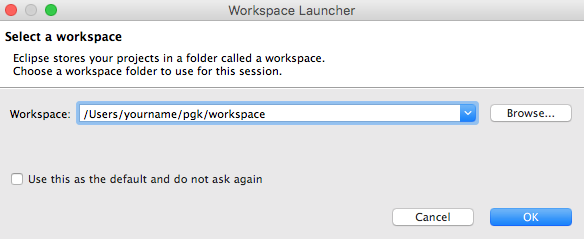
\includegraphics[width=0.7\textwidth]{../img/pirates/selectws.png}
\caption { \emph{Öppna workspace:} Bläddra fram till kursens workspace och klicka {\bf OK. }}
\label{fig:eclipse:ide:open}
\end{figure}

\item Gå vidare från startskärmen genom att välja {\bf Workspace}, se Fig.\ref{fig:eclipse:ide:selectws}.
\begin{figure}[H]
\centering
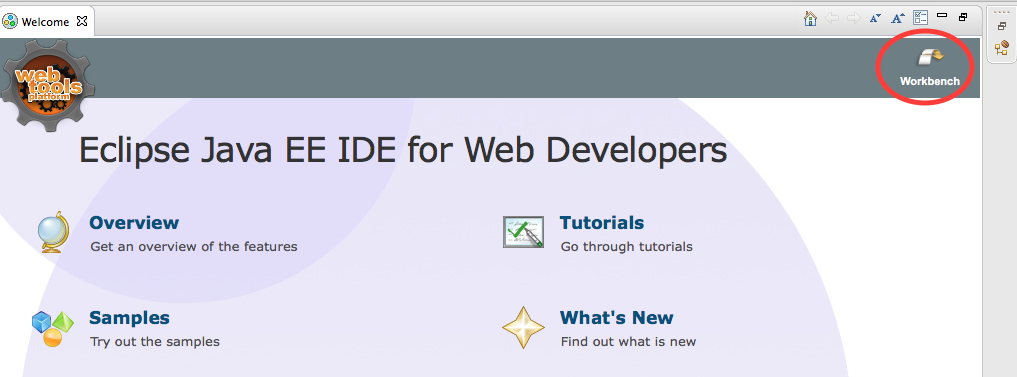
\includegraphics[width=0.7\textwidth]{../img/pirates/selectws2.png} \\

\caption {Välj {\bf workspace}.}
\label{fig:eclipse:ide:selectws}
\end{figure}

\item Uppe till höger ser du vilken \emph{vy} du har. I Eclipse kommer vi växla mellan Scala, Java och debug-vyer. Dessa läggs till via listan som nås genom den fönsterliknande ikonen enligt Fig.~\ref{fig:eclipse:ide:changeview}. Du ska ha {\bf Scala} igång.

\begin{figure}[H]
\centering
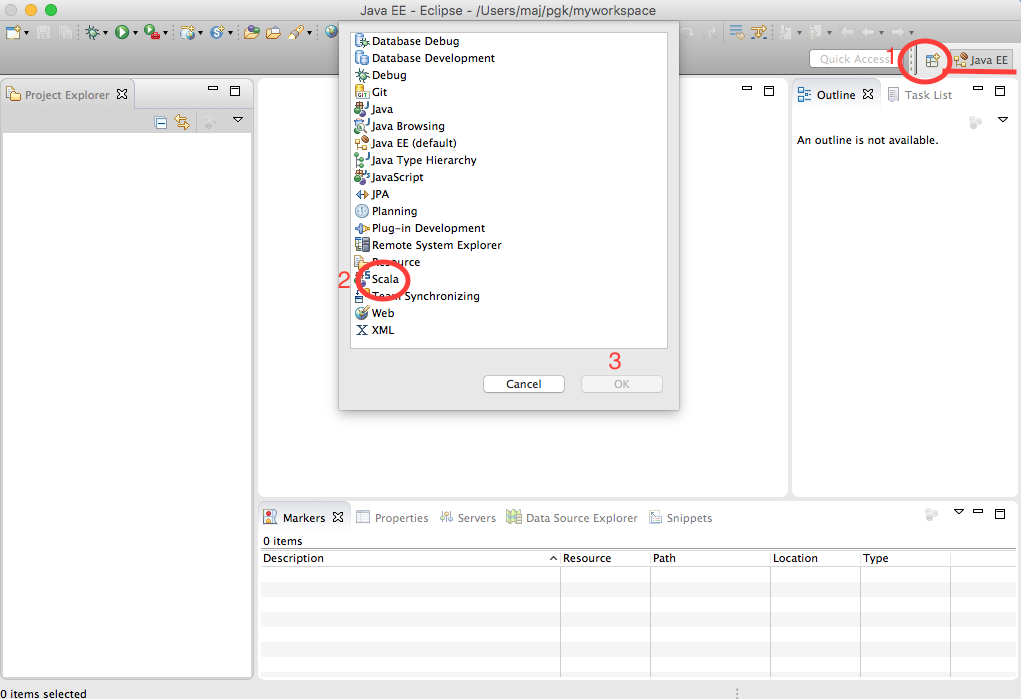
\includegraphics[width=0.7\textwidth]{../img/pirates/selectscala.png} 

\caption {Lägg till vyer från listan med installerade plugin.}
\label{fig:eclipse:ide:changeview}
\end{figure}

\item Högerklicka i {\bf Project Explorer} och välj {\bf New} -> {\bf Scala Project}, se Fig.~\ref{fig:eclipse:ide:createproject}. Importera existerande project genom att genom att avmarkera \emph{Use default location} och bläddra till katalogen för respektive laboration och sen {\bf Finish}, se exempel i Fig.~\ref{fig:eclipse:ide:import} (namnet sätts automatiskt). Du kan också skapa nya projekt genom att ange ett projektnamn direkt och sen klicka {\bf Finish} enligt Fig.~\ref{fig:eclipse:ide:newproject}.

\begin{figure}[H]
\centering
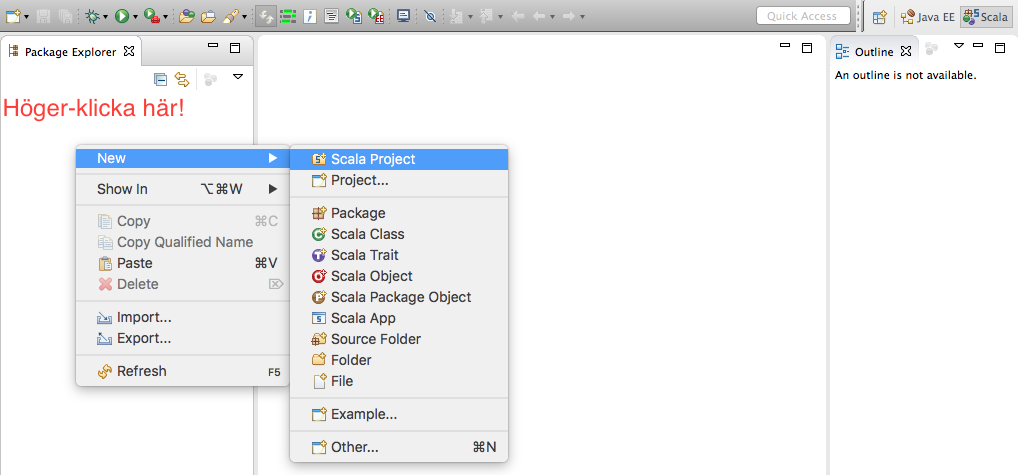
\includegraphics[width=0.7\textwidth]{../img/pirates/createproject.png} 

\caption {Välj att {\bf Scala Project} i menyerna.}
\label{fig:eclipse:ide:createproject}
\end{figure}
\begin{figure}[H]
\centering
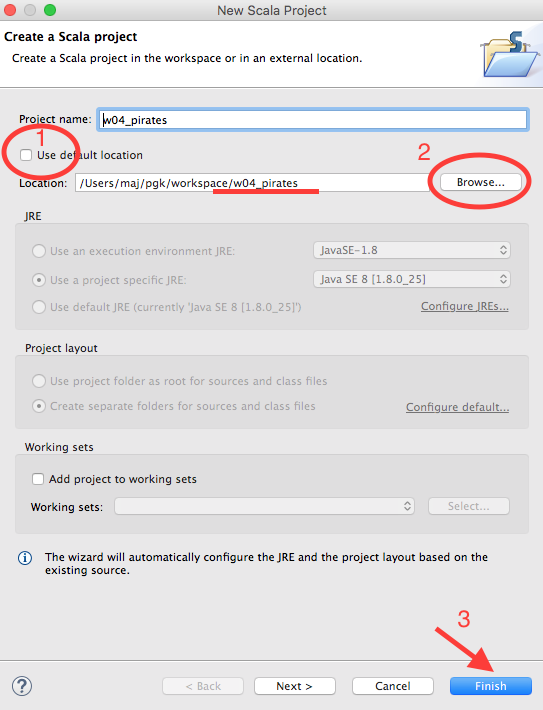
\includegraphics[width=0.5\textwidth]{../img/pirates/importproject.png} 

\caption {Importera existerande projekt genom att ange sökvägen.}
\label{fig:eclipse:ide:import}
\end{figure}

\begin{figure}[H]
\centering
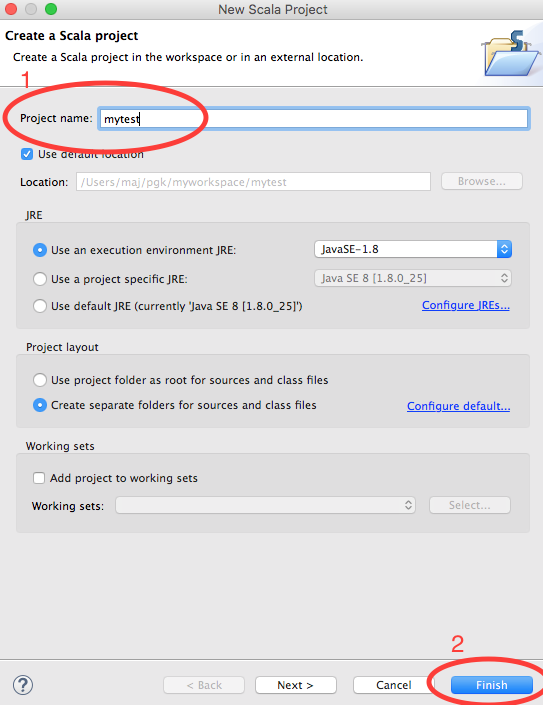
\includegraphics[width=0.5\textwidth]{../img/pirates/nameproject.png} 

\caption {Skapa ett nytt projekt genom att ange namn.}
\label{fig:eclipse:ide:newproject}
\end{figure}


\item Du skapar nya klasser och objekt på liknande sätt, genom att högerklicka och välja {\bf New}, se exempel i Fig.~\ref{fig:eclipse:ide:createobject}


\begin{figure}[H]
\centering
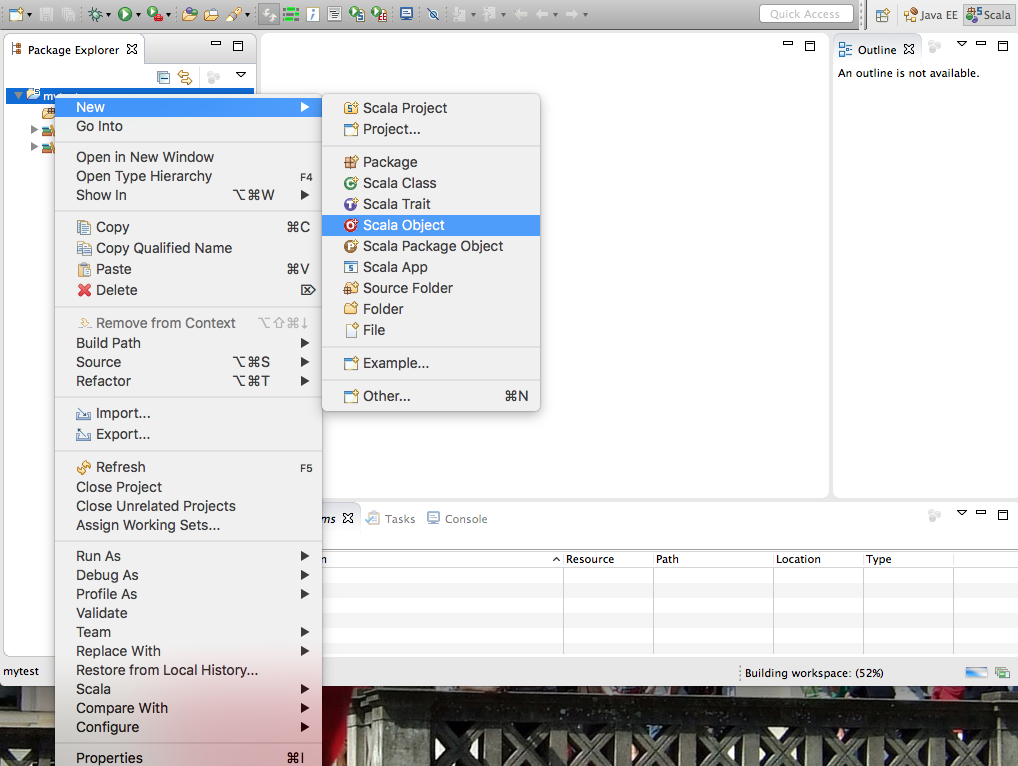
\includegraphics[width=0.7\textwidth]{../img/pirates/createobject.png} 
\caption {Skapa ett nytt objekt via menyerna.}
\label{fig:eclipse:ide:createobject}
\end{figure}

\item Skriv ett main-program och exekvera det genom att markera klassen i {\bf Project Explorer} och sen klicka på den gröna pilen. Utskrifter kommer till konsolen längst ner. 

\begin{figure}[H]
\centering
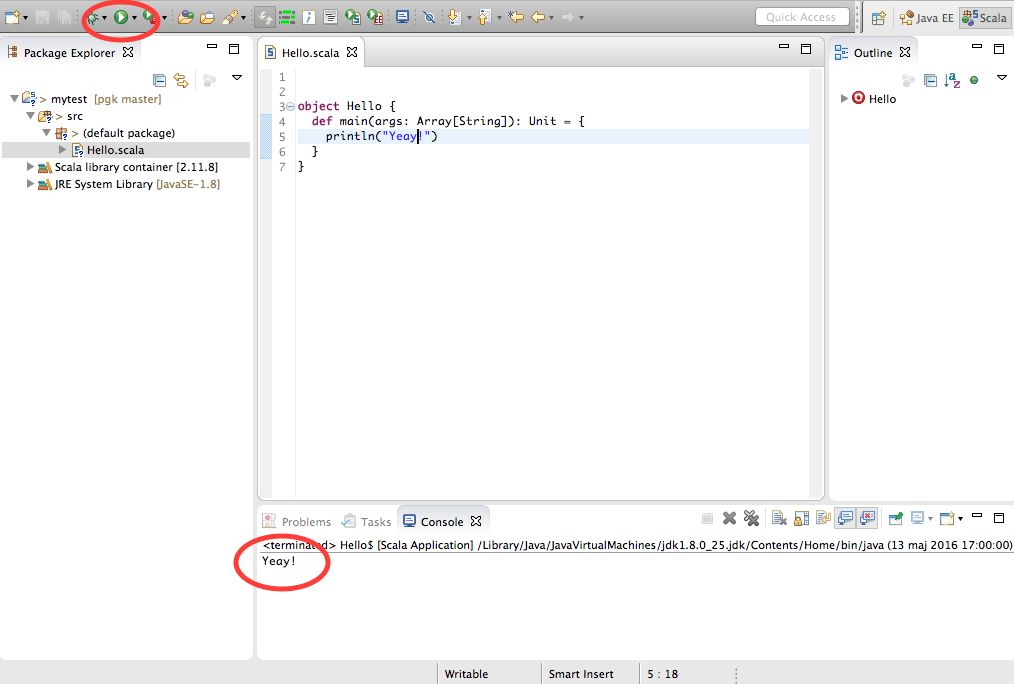
\includegraphics[width=0.7\textwidth]{../img/pirates/exekvera.png} 
\caption {Exekvera med den gröna pilen.}
\label{fig:eclipse:ide:exec}
\end{figure}
\end{itemize}



